%%%%%%%%%%%%%%%%%%%%%%%%%%%%%%%%%%%%%%%%%%%%%%%%%%%%%%%%%%%%
% Paul McKee
% Rensselaer Polytechnic Institute
% 1/31/18
% Master's Thesis
% with Dr. Kurt Anderson
% LaTeX Template: Project Titlepage Modified (v 0.1) by rcx
%%%%%%%%%%%%%%%%%%%%%%%%%%%%%%%%%%%%%%%%%%%%%%%%%%%%%%%%%%%%

\documentclass[12pt]{article}

%\usepackage[demo]{graphicx}
\usepackage{caption}
\usepackage{subcaption}

\usepackage{blindtext}
\usepackage[utf8]{inputenc}

\usepackage{graphicx, wrapfig, subcaption, setspace, booktabs}
\usepackage{sectsty}
\usepackage{url, lipsum}
\usepackage{makecell}
\usepackage{amsmath}
\usepackage{setspace}
\usepackage{amsmath}
\usepackage{color} %red, green, blue, yellow, cyan, magenta, black, white
\definecolor{mygreen}{RGB}{28,172,0} % color values Red, Green, Blue
\definecolor{mylilas}{RGB}{170,55,241}

\usepackage[table,xcdraw]{xcolor}


\usepackage[margin=.75in]{geometry} 
\usepackage{amsmath,amsthm,amssymb}
\usepackage{color}
\usepackage{fancyhdr}
\usepackage{lastpage}
\usepackage{graphicx}

\usepackage{cite}%AddedbyChris
\usepackage{graphicx}%AddedbyChris
\usepackage{array}%Added by Chris
\usepackage{caption}
\usepackage{amsmath}%Added by Chri
\pagestyle{fancy}
\fancyhf{}
%\fancyhead[L]{Independant Study}
%\fancyhead[C]{\rightmark}
\fancyhead[C]{}

\fancyhead[L]{\nouppercase{\leftmark}}
\fancyhead[R]{Philip Hoddinott}

\rfoot{Page \thepage \hspace{1pt} of \pageref{LastPage}}

\newcommand{\N}{\mathbb{N}}
\newcommand{\Z}{\mathbb{Z}}
\newcommand{\norm}[1]{\left\lVert#1\right\rVert}

\newenvironment{theorem}[2][Theorem]{\begin{trivlist}
		\item[\hskip \labelsep {\bfseries #1}\hskip \labelsep {\bfseries #2.}]}{\end{trivlist}}
\newenvironment{lemma}[2][Lemma]{\begin{trivlist}
		\item[\hskip \labelsep {\bfseries #1}\hskip \labelsep {\bfseries #2.}]}{\end{trivlist}}
\newenvironment{exercise}[2][Exercise]{\begin{trivlist}
		\item[\hskip \labelsep {\bfseries #1}\hskip \labelsep {\bfseries #2.}]}{\end{trivlist}}
\newenvironment{problem}[2][Problem]{\begin{trivlist}
		\item[\hskip \labelsep {\bfseries #1}\hskip \labelsep {\bfseries #2.}]}{\end{trivlist}}
\newenvironment{question}[2][Question]{\begin{trivlist}
		\item[\hskip \labelsep {\bfseries #1}\hskip \labelsep {\bfseries #2.}]}{\end{trivlist}}
\newenvironment{corollary}[2][Corollary]{\begin{trivlist}
		\item[\hskip \labelsep {\bfseries #1}\hskip \labelsep {\bfseries #2.}]}{\end{trivlist}}

\newenvironment{solution}{\begin{proof}[Solution]}{\end{proof}}
\usepackage{multicol}
\newcommand{\mysize}{0.5}
\usepackage{subcaption}
\usepackage{float}
\usepackage{listings}
\usepackage{color} 
\newcolumntype{L}{>{\centering\arraybackslash}m{3cm}}
\usepackage{setspace}
\usepackage[framed,numbered,autolinebreaks,useliterate]{mcode}

\newlength\longest

% %---------------------------------------------------------------
% % HEADER & FOOTER
% %---------------------------------------------------------------

%\fancyhf{}
%\pagestyle{fancy}
%\renewcommand{\headrulewidth}{0pt}
%\setlength\headheight{0pt}
%\fancyhead[L]{ Paul McKee }
%\fancyhead[R]{Rensselaer Polytechnic Institute}
%\cfoot{ \thepage\ } 


%--------------------------------------------------------------
% TITLE PAGE
%--------------------------------------------------------------
\iffalse
\begin{titlepage}
	\title{ 
		\LARGE \textbf{\uppercase{Put Title Here}} \\
		\vspace{0.25cm}
		\LARGE \textbf{Philip Hoddinott}
	}
	\author{\small{Submitted in Partial Fulfillment of the Requirements} \\ \small{for the Degree of} \\
		\uppercase{Master of Science} \\ \\
		Approved by:
		\\ Kurt Anderson, Chair \\ John Christian \\ Matthew Oehlschlaeger \\ \\ %% from paul's template
		\includegraphics[width=2.5cm]{rensselaer_seal.png} \\
		\small{\textit{Department of Mechanical, Aerospace, and Nuclear Engineering}} \\
		\small{Rensselaer Polytechnic Institute} \\ 
		\small{Troy, New York} \\
		\small{November 2018}
	}
\end{titlepage}
\fi

\begin{document}
		\title{Deep Neural Network}
	\author{Philip Hoddinott}
	
	\maketitle
	%\pagenumbering{roman}
	%\thispagestyle{empty}
	%\clearpage


	
	%\newpage


	%\thispagestyle{fancy}
	
	%\addcontentsline{toc}{section}{\uppercase{Table of Contents}}
	%\listoftables
	%\addcontentsline{toc}{section}{\uppercase{List of Tables}}
	%\listoffigures
	%\addcontentsline{toc}{section}{\uppercase{List of Figures}}
	% -----------------------------
	
	% ------------------------------------------------------------
	% Acknowledgement
	% ------------------------------------------------------------



	
	% ------------------------------------------------------------
	% Abstract 
	% ------------------------------------------------------------
	
	\newpage
	\section*{Abstract}
	\textcolor{red}{Remove pasive voice, will, chec out rubirc }
	The purpose of this report is to develop a neural net that can identify handwritten digets in the MNIST database at near human levels of accuracy. The neural net will be developed without the assistance of libraries such as Python's tensor flow or MATLAB's Deep Learning. 
	
	solve the MNIST  on the mnist database
	. \par 
	The author would like to express his gratitude to Professor Hicken
	
	
	 for his suggestion of this project and his assistance with the methods of orbital determination through out the semester.\par 
	
		\newpage
%\setcounter{page}{1}
\tableofcontents
\listoffigures
\doublespacing
	%\textcolor{red}{ Do More}
	% ------------------------------------------------------------
	% Introduction
	% ------------------------------------------------------------
	\newpage
	 % this should start the normal numberinbg

	\section{Introduction}
	Have it solve the MNIST with a simple simple thing
	then try diffrent layers and stuff
	
	Go over tan h vs sigmoid\
	Explain batch testing
	
	\subsection{Background}
	\subsection{The MNIST database}
	The Modified National Institute of Standards and Technology database or MNIST database\cite{mnistDATABASE} is a database of handwritten numbers used to train image processing systems. It contains 60,000 training images and 10,000 testing images. 
	
	A number of attempts have been made to get the lowest possible error rate on this dataset. As of August 2018 the  the lowest achieved so far is a error rate of 0.21\% or an accuracy of 99.79\%.  For comparison human brains that are hardwired for pattern recogntion 1.5 \textcolor{red}{Come back to}\cite{humanPerf}.
	
	The database is comprised of images that are made up of a grid of 28x28 pixels, as seen in figure \ref{fig:mathworksmnistneuralnetfinal}. 
	
	\begin{figure}[H]
		\centering
		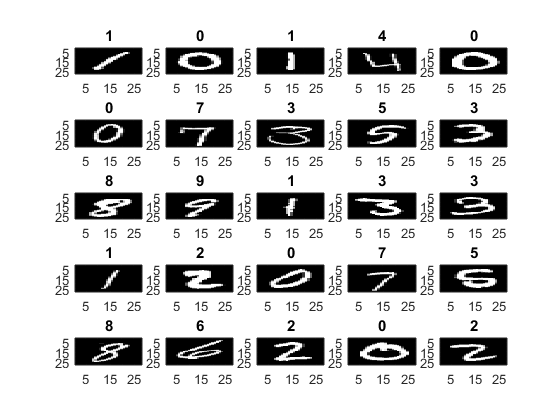
\includegraphics[width=0.7\linewidth]{mathworks_mnist_neuralnetFinal}
		\caption{Sample numbers from MNIST \cite{matlabNNBeg}.}
		\label{fig:mathworksmnistneuralnetfinal}
	\end{figure}
	
	\subsection{Artificial neural network}
	An artifical nerual nework (refered tp as a NN in this paper)
	
	\subsubsection{Forward Propgation}
	\subsubsection{Back propgration}
	
	\subsubsection{activation function}
	
	Tan h
	The derivative of tanh is seen in equation \ref{eqn:dtanh}
	\begin{equation}
	\phi'(z)=\frac{4}{\left(x^{-z}+e^{z}\right)^2}
	\label{eqn:dtanh}
	\end{equation}
	Sigmoid
	The sigmoid function is senn in 
	
	
	\begin{equation}
	\phi(z)=\frac{1}{1+e^{-z}}
	\label{eqn:sig}
	\end{equation}
	The deritvative of the sigmoid function is
	\begin{equation}
	\phi'(z)=\frac{e^{-z}}{\left(e^{-z}+1\right)^2}
	\end{equation}
	Expalain importance of activation function
	
	\subsubsection{Pitfalls}
	The most important thing to stear clear of is over traning. Overtraning occurs when the neural net trains too much to the traning data. While it will have a high accuracy for the traning data, it's performance for the test data will decay, as it has become too well attuned to the trainting data.  \par 
	
	The other problem is the time it takes to train. A three layer neural net can be trained to 97\% accurcy within 10 minutes, however it will not improve far beyond that. Larger nets will take longer to train, but will take far longer to train. 
	
	\begin{figure}
		\centering
		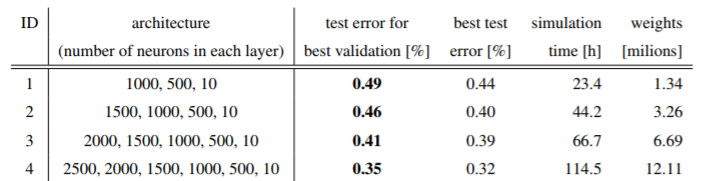
\includegraphics[width=0.7\linewidth]{nnRunTime}
		\caption{Run times for various neural network architectures\cite{deepBig}.}
		\label{fig:nnruntime}
	\end{figure}
	
	\section{Implementation}
	
	
	Go over how it was implemented
	Go over batch testing
	
	restuls, comparison of diffrent arctiectures
	
	Go over the way this was implmented for the best way
	
	
	
	
	\section{Results}
	\subsection{Simple Nerual Net}
	
	
	 %, Kepler, Newton, and Euler\cite{lectureOnGreekAstro}. 
	
	%\textcolor{red}{Segway hre}


	
	\section{Conclusion}

			%--------------------------------------
		% References
		% -------------------------------------
		
		\bibliographystyle{unsrt}
		\bibliography{ref}

		
		%-----------------------------------------------------------
		% Appendix
		%-----------------------------------------------------------
		\newpage
		\singlespacing
%		\section*{Appendix 1 -derivation of gibbs}
		\section*{Appendix 1 - MATLAB code}
		\addcontentsline{toc}{section}{Appendix}
		
		\lstset{language=Matlab,%
			%basicstyle=\color{red},
			breaklines=true,%
			morekeywords={matlab2tikz},
			keywordstyle=\color{blue},%
			morekeywords=[2]{1}, keywordstyle=[2]{\color{black}},
			identifierstyle=\color{black},%
			stringstyle=\color{mylilas},
			commentstyle=\color{mygreen},%
			showstringspaces=false,%without this there will be a symbol in the places where there is a space
			numbers=left,%
			numberstyle={\tiny \color{black}},% size of the numbers
			numbersep=9pt, % this defines how far the numbers are from the text
			emph=[1]{for,end,break},emphstyle=[1]\color{red}, %some words to emphasise
			%emph=[2]{word1,word2}, emphstyle=[2]{style},    
		}
	%\lstinputlisting{C:/Users/Philip/Documents/GitHub/Thesis/Master_TLE.m}
	%\lstinputlisting{C:/Users/Philip/Documents/GitHub/independent_study_fall_2018/Independat-Study-Fall-2018/Gibbs_Heck_master_loop_Latex.m}
	
	%\subsection{Code}
	%\subsection{Master\_TLE.m}
	%\lstinputlisting{C:/Users/Philip/Documents/GitHub/Thesis/Master_TLE.m}
	%\subsection{get\_SATCAT.m}
	%	\lstinputlisting{C:/Users/Philip/Documents/GitHub/Thesis/get_SATCAT.m}
	%	\subsection{get\_TLE\_from\_ID\_Manager.m}
	%\lstinputlisting{C:/Users/Philip/Documents/GitHub/Thesis/get_TLE_from_ID_Manager.m}
	
	%\subsection{get\_TLE\_from\_NorID.m}
	%\lstinputlisting{C:/Users/Philip/Documents/GitHub/Thesis/get_TLE_from_NorID.m}
	%\lstinputlisting{get_SATCAT.m}
	
	%Thanks for Paul McKee who started this template. It seems to have good matlab code viwing
		
	\end{document}
	
